\chapter{Subsystem Implementation\label{cha:implementation}}

The purpose of this chapter is to document the work completed in the implementation phase of the project. During this phase of the project, we had three major goals in mind:
\begin{enumerate}
  \item The implementation's primary objective is to verify the system design, and compare the results with those desired in Ch. \ref{cha:goals}.
  \item The implemented systems are to be used as working prototypes for demonstration and communication of various aspects of the project.
  \item Finally, it was desired to produce a first iteration of usable modules for the Formula SAE team to integrate into the vehicle and take to competition in May, 2010.
\end{enumerate}

This chapter is broken down into four sections: first the simulation and physical implementation of the electro-pneumatic subsystem is discussed, followed by sections on the hardware and software implementations of the 4 modules. Finally, a section is devoted to the CAN Snooper and Injector, which was implemented to permit easier in-place testing of modules individually and together.

\section{Electro-Pneumatic System\label{sec:electropneumatic_implementation}}

\nomenclature{PID}{Proportional-Integral-Differential}

Several steps were taken in the implementation phase to develop a better understanding of the electro-pneumatic's behaviour, and to provide data and models that could be used in the implementation of the controller software. A Simulink model was developed to verify that our fundamental design would work, and to gain further insight into the operation of the electro-pneumatic system. A simple \emph{Proportional-Integral-Derivative} (PID) controller block was used to show that the closed-loop system was inherently stable.

\subsection{Simulation with Simulink}

An overview of the Simulink model used to simulate the electro-pneumatics system is shown in \ref{fig:pneumatics_top_level}. A PID controller block is used in a closed-loop configuration, and the response to a fixed step input is displayed on the scope block. 

\begin{figure}[H]
\centering
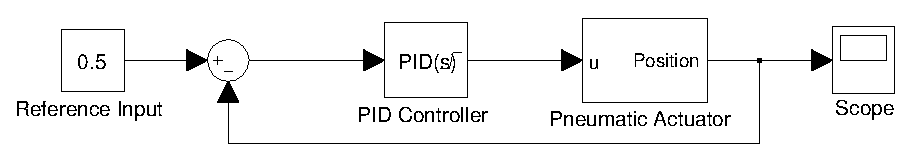
\includegraphics[scale=1]{implementation/figures/pneumatic_modelling1.eps}
\caption{Simulink model of the electro-pneumatic system.}
\label{fig:pneumatics_top_level}
\end{figure}

The three major components of the electro-pneumatic system are the \emph{PWM generator}, the \emph{solenoid valves}, and the \emph{pneumatic actuator}. Models of these systems are described further in the following sections.

\subsubsection{PWM Generator Model}

The PWM generator is used to provide the electrical control signals required by the solenoid valves to open and close. Our model of the PWM generator uses the instantaneous model presented by \citet{valve_models}. This model compares a generated saw-tooth signal $V_{saw}$ with the input signal $V_{in}$ over a time period $T_{saw}$ to obtain the pulse-width-modulated signal $U(t)$. The relationship is illustrated in Eq. \ref{eq:pwm_generation}.

\begin{equation}
\label{eq:pwm_generation}
U\left(t\right) = 
\begin{cases}
1 & V_{in}\left(t\right) \geq V_{saw}\left(t\right) \\
0 & V_{in}\left(t\right) < \left(t\right)
\end{cases}
\end{equation}

The Simulink model which implements Eq. \ref{eq:pwm_generation} can be seen in Fig. \ref{fig:pneumatics_pwm}. The input to the subsystem, shown as \emph{In1}, is $V_{in}$, and the output, shown as \emph{Out1} is the pulse width modulated signal $U(t)$. 

\begin{figure}[H]
\centering
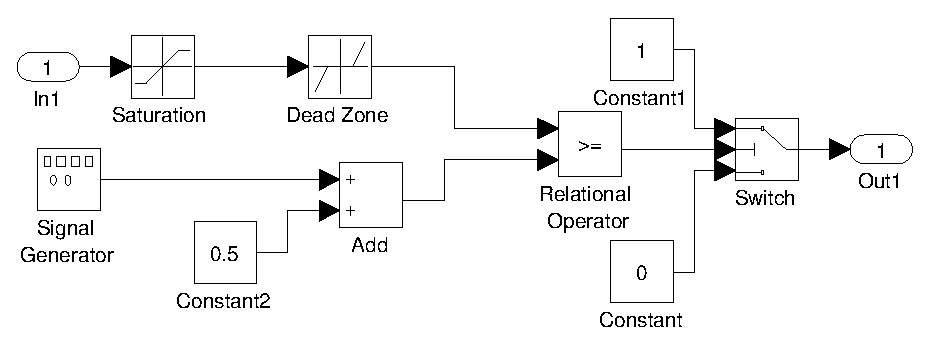
\includegraphics[scale=0.65]{implementation/figures/pneumatic_modelling2.eps}
\caption{Simulink model of the PWM generator.}
\label{fig:pneumatics_pwm}
\end{figure}

A saturation block limits the input signal $V_{in}$ to the range of \unit{[0..1]}{\volt}. A dead-zone block is present to account for the dead-zone present in the solenoid valve response to a PWM signal. If the pulse width is too short, the current through the solenoid cannot generate enough force to open the poppet, so the valve stays shut. This is a parameter of the solenoid valve, and was quantified experimentally by \cite{valve_models} as the minimum input signal $V_{in}$ required to open the valve. \Citet{accurate_position} also account for a minimum possible duty cycle in the solenoid valve input signal, known as $d_{min}$. This value can be calculated as:

\begin{equation}
  \label{eq:pwm_duty_min}
  d_{min}=\left(T_{vr}/T_{PWM}\right)\cdot100\%
\end{equation}

In this case, $T_{vr}$ is the time required by a solenoid valve to respond to an input, and $T_{PWM}$ the period of the PWM signal.

\nomenclature{$d_{min}$}{The minimum possible duty cycle of a solenoid's drive signal that will cause the valve to open.}
\nomenclature{$T_{vr}$}{The time required by a solenoid valve to respond to an input.}

The signal generator block in Fig. \ref{fig:pneumatics_pwm} outputs a triangle wave with peak-to-peak amplitude of \unit{1}{\volt}, which is then offset by \unit{0.5}{\volt}. The relational operator block then compares this with the input signal, and outputs the resulting PWM signal.

\subsubsection{Solenoid Valve Model}

An initial Simulink model of a solenoid valve was constructed based on the modelling equations described by \citet{valve_models} and the standard orifice equations for laminar and choked flow described in \cite{fluid_power}. However, it was too difficult to identify the system parameters cited in \cite{fluid_power} for our specific solenoid valves. The solenoid's data-sheet was not detailed enough, and the straight-forward approach to system identification used by \cite{valve_models} required specialized measuring equipment (such as an instantaneous mass flow meter) that we did not have access to.

The custom Simulink solenoid valve block was replaced with an approximate Simulink ``Simscape'' pneumatic valve block. This block could be configured with data obtained from the valve's data-sheets. 

\subsubsection{Pneumatic Actuator Model}

Simulink's pneumatic actuator subsystem is illustrated in Fig. \ref{fig:pneumatics_actuator}. Pre-built Simulink blocks from the Simscape package were used to model the dynamics of the actuator. \emph{Physical Port 1} (denoted by the octagonal port symbol with a ``1'' inside) in \ref{fig:pneumatics_actuator} represents the air inlet. \emph{Physical Ports 2 and 3} (denoted by the octagonal port symbols with a ``2'' and ``3'' inside, respectively) represent the displacement ports of the cylinder. \emph{Regular Port 1} (denoted by the rounded port symbol with a ``1'' inside) is used to display the displacement on a scope.

\begin{figure}[H]
\centering
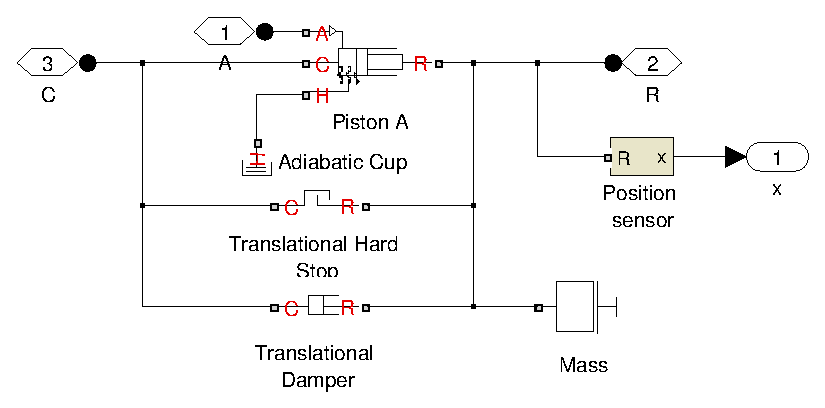
\includegraphics[scale=0.65]{implementation/figures/pneumatic_modelling3}
\caption{Simulink model of the pneumatic actuator.}
\label{fig:pneumatics_actuator}
\end{figure}

\subsubsection{Integrated Simulink Model}

The complete open-loop actuator model can be seen in Fig. \ref{fig:pneumatics_model_full}. The absolute value of the real-valued input $u$ is first fed to the PWM block. This signal is then converted into separate signals for each of the two solenoid valves in a way similar to the first PWM pulsing scheme presented by \citet{accurate_position}. The input to the subsystem $u$ is expected to range from -1 to 1. When $u\geq0$, the input to valve A is the pulse width modulated signal $U$, and the input to valve B is 0. When $u<0$, the opposite situation occurs.

\begin{figure}[H]
\centering
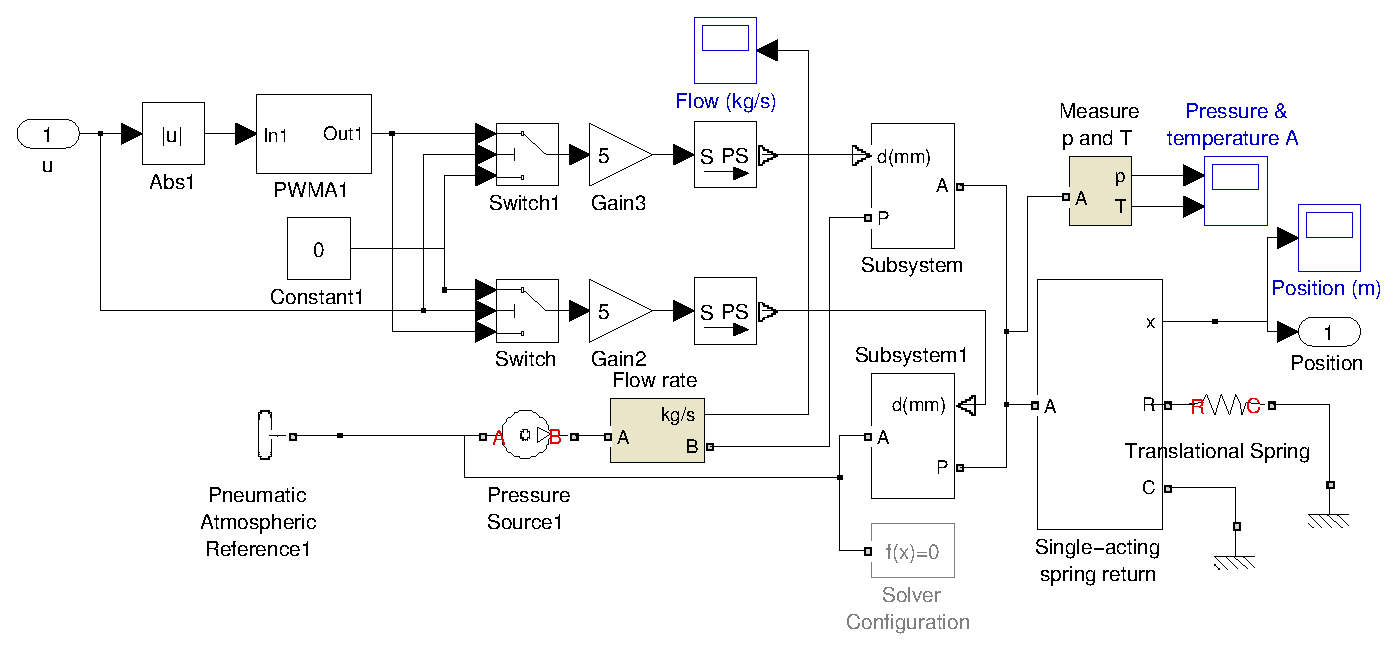
\includegraphics[scale=0.65]{implementation/figures/pneumatic_modelling4}
\caption{Simulink model of the full electro-pneumatic system.}
\label{fig:pneumatics_model_full}
\end{figure}

\subsection{Component Selection}

Selection of components was limited by budgetary constraints, however adequate solenoid valves and pneumatic actuators were found. These are detailed in the following sections.

\subsubsection{Solenoid Valves}

Solenoid valves and cylinders from SMC corp were chosen for the physical implementation of the design, specifically the \emph{VQZ115} series valve. Table \ref{tab:solenoid_specs} shows the specifications for this solenoid valve. A maximum operating frequency of \unit{20}{\hertz} was the fastest available solenoid that met the output force requirements while still being within the Formula SAE budget.

\begin{table}[H]
  \caption{Specifications of the SMC VQZ115 solenoid valve.\label{tab:solenoid_specs}}
  \centering

  \begin{tabular}{|l|l|}
  \hline
  Part & VQZ115-6L1-N1-PR \tabularnewline
  \hline
  Coil Voltage & \unit{12}{\volt} \tabularnewline
  \hline
  Configuration & 3-port Normally Closed \tabularnewline
  \hline
  Flow Coefficient & $C_v=\unit{0.23}{}$ \tabularnewline
  \hline
  Maximum Operating Frequency & \unit{20}{\hertz} \tabularnewline
  \hline
  Maximum Pressure & \unit{0.7}{\mega\pascal} \tabularnewline
  \hline
  \end{tabular}
\end{table}

\subsubsection{Pneumatic Actuators}

The pneumatic actuators specified for implementation are the same as used in the previous design, and are only briefly mentioned in this report. Specifications can be found in Table \ref{tab:cylinder_specs}. The clutch cylinder is specified with an internal magnet on the piston that interfaces magnetically with a membrane potentiometer, discussed next.

\begin{table}[H]
 \caption{Specifications of the pneumatic actuators used.\label{tab:cylinder_specs}}
  \centering
  \begin{tabular}{|l|l|l|l|}
   \hline
   Part & Bore Size & Stroke & Part Number \tabularnewline
    \hline
    \hline
    Shift actuator & 9/16`` & 2'' & NCMC056-0200 \tabularnewline
    \hline
    Clutch actuator & 3/4`` & 2'' & NCDMC075-0200 \tabularnewline
    \hline
  \end{tabular}
\end{table}

\subsubsection{Positional Feedback Sensors}

A ``MagnetoPot'' contact-less potentiometer from Spectra Symbal provides positional feedback from the clutch cylinder. The internal magnet in the cylinder interacts with the ``MagnetoPot'', which has a three-wire electrical interface similar to a standard potentiometer.


\section{Hardware Implementation\label{sec:Hardware-Implementation}}


\subsection{Methodology}

Commonality between modules, same life-support system.


\subsection{CAD Design}

Schematic capture and PCB layout using EagleCAD.


\subsection{Commonalities}

All 4 modules are implemented on custom printed circuit boards (PCBs) with an \emph{AT90CAN128} micro-controller from Atmel. Programming and debugging software on the microcontroller was done through a standard IEEE 1149.1 JTAG interface. The module is linked to the other system modules with a CAN bus. All inter-module communication is done over the CAN bus.

\subsubsection{Microcontroller}


\subsubsection{CAN Transceiver}


\subsubsection{Linear Regulator}


\subsubsection{Supervisor}


\subsubsection{Wiring Harness}


\subsection{Engine and Transmission Module}

<Picture of board>

Overview of physical implementation.


\subsubsection{High Current Solenoid Driver}


\subsubsection{Input Buffers}


\subsubsection{Traction Control Analogue Output}

The ECU allows a 0-5v analogue input to modify the allowable traction slip ratio from 0-100\% for the traction control.

The Engine module uses a simple SPI interfaced DAC from Texas Instruments, the TLV5623, to output the 0-5v analogue signal to the ECU.

The output voltage from the DAC is given by

\begin{equation}
V_{out}=2\cdot{V_{ref}}\,\frac{Code}{2^{n}}\,[V]
\end{equation}

where $V_{ref}$ is the reference voltage input to the chip, $n=8\,(bits)$, and $Code$ is the digital input value ranging from $0$ to $2^{n-1}$. Since we want to output $5\,[V]$ at fullscale input, \begin{equation} 2\cdot{V_{ref}}\,\frac{2^{7}}{2^{8}}=V_{ref}=5\,[V]\end{equation}.

The DC input resistance $R_{in}$ on the traction cut input pin on the ECU was measured using a series resistor with the input terminal to be $R_{in}\approx155k\Omega$. The output current of the DAC therefore will be at most $I_{out}=\frac{5v}{155k}\approx32.26\mu A$.

\subsection{Braking Module}

\begin{figure}[h]
\centering
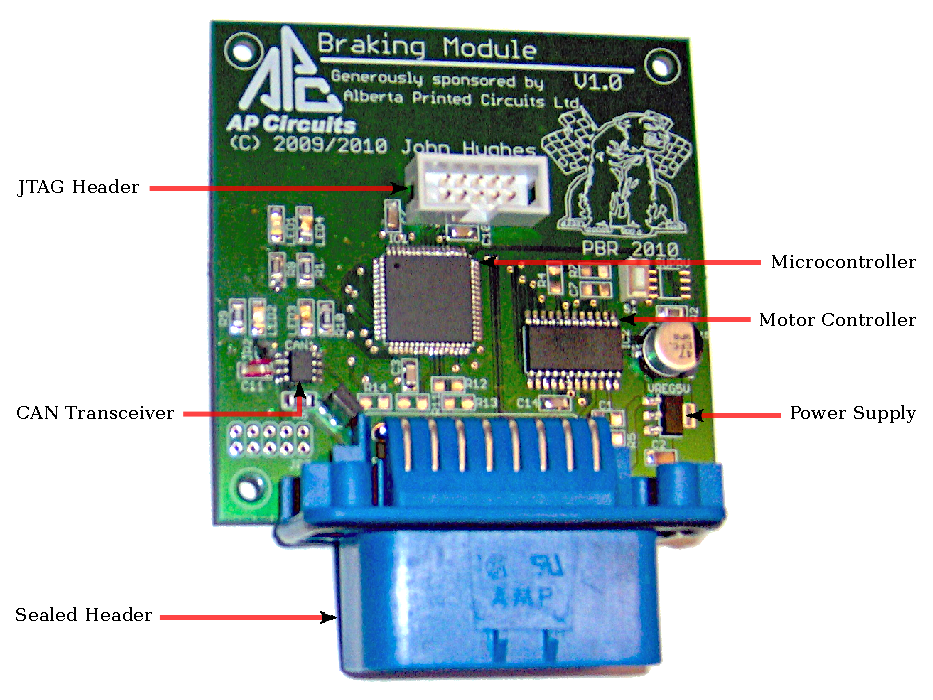
\includegraphics[scale=1]{implementation/figures/braking_pcb}
\caption{Populated Braking module PCB.}
\label{fig:braking_pcb}
\end{figure}

The braking module implementation was the simplest of the 4 modules in terms of electrical design. Only one special component on the board was required, a stepper motor controller/driver, and the interface to the microcontroller only required a handful of i/o lines. Additionally, a pressure transducer was also specified to facilitate measuring the hydraulic pressure in the brake lines. The components chosen for the braking module are listed in Table \ref{table:braking_module_components}.

Figure \ref{fig:braking_pcb} shows a photograph of the completed braking module circuit board, with all components soldered on. The simplicity of the electrical design is reflected in the fact that no additional corrections (other than for the CAN transceiver) were required for the module to be 100\% operational.

\begin{table}
  \caption{Braking module components.\label{table:braking_module_components}}
  \centering
  \begin{tabular}{|c|c|c|}
    \hline 
    Part & Manufacturer & Part Number\tabularnewline 
    \hline \hline
    Stepper Motor Controller/Driver & Allegro Microsystems & A3967 \tabularnewline
    \hline
  \end{tabular}
\end{table}

\subsubsection{Stepper Motor Driver}

In order to meet the design goal of having the implementation be flexible in terms of which stepper motor would be used in the system, a current-sensing stepper motor controller/driver component was used in the circuit design. The current sense capability allows us to fix the input voltage in the circuit design, and afterwards adjust the current drive by changing resistor values in the current-sense feedback loop. 

The A3967 "Microstepping Driver with Translator" was chosen to drive the stepper motor for several reasons. The A3967 integrates a microstepping controller with dual H-Bridge output stages into one package. This simplified the potential circuit design. The H-Bridge output transistors can supply up to $\pm\unit{750}{\milli\ampere}$ of current at up to \unit{30}{\volt} \cite{A3967}. This flexibility was desirable.

\paragraph{Current Control}
\nomenclature{$R_{sense}$}{Value of the current sense resistors in the Braking Module's stepper motor circuit.}
\nomenclature{$I_{TRIP}max$}{Maximum current allowed to flow into the Braking Module's stepper motor before the PWM circuit shuts the output stage off.}

The current control feature of the A3967 works by sensing the current through a sense resistor, $R_{sense}$, and varies the duty cycle of a fixed off-time PWM circuit, which controls the output from the H-Bridge stages.

The value of the sense resistor was determined by an equation recommended in the datasheet:
\begin{equation}
R_{sense}=\frac{0.5}{I_{TRIP}max}
\end{equation}
where $I_{TRIP}max$ is the maximum current allowed to flow into the motor before the PWM circuit shuts the output stage off.

\subsubsection{Analogue-to-Digital Converter}


\subsubsection{End-of-Travel Microswitches}

\subsection{Telemetry Module}


\subsubsection{Wireless Modem}

To meet the range and data throughput requirements for the telemetry system, an XBee Pro wireles modem was used. The XBee requires 3.3v I/O levels and power supply, and so a second linear voltage regulator was used in the design, the LT1521 from Linear Technology. Since the AT90CAN129 has only 2 built-in UARTS that were used for the RS232 interfaces to the ECU and DAQ, an third external UART was added to the design. The MAX3100 is a SPI-interfaced UART with an 8 word deep FIFO buffer. It is interfaced to the AT90CAN128's SPI pins and has an active-low IRQ line connected to external interrupt line EXT7 on the microcontroller. 

The wireless transmitter is an XBee Pro Modem from Digi International. The modem is in a package designed for mounting on a printed circuit board, and is attached to the telemetry module directly. This modems requires a 3.3V power supply. and consumes at most 215mA of current during transmit. Since the common module hardware only provides power for 5V devices, the telemetry module has a second LDO regulator providing 3.3V. A separate antenna port is connected to the modem and mounted in the side of the module enclosure.



\subsubsection{External SPI USART}


\subsubsection{Two-Channel ECU and DAC USART}

\subsection{Driver Interface Module}


\subsubsection{Steering Wheel Unit}


\subsubsection{LCD Module Bias Circuit}

The LCD screen requires a large bias voltage of +22V.

A Linear Technology LT1615 step-up DC/DC converter was chosen as the centre of a boost converter circuit for the LCD.


\paragraph{Inductor Selection}

\begin{equation}
L=\frac{V_{out}-V_{in(min)}+V_{D}}{I_{limit}}\cdot t_{off}\label{IndSel}
\end{equation}


Using (\ref{IndSel}) with $V_{D}=0.4V$, $I_{limit}=350mA$, $t_{off}=400ns$, $V_{out}=+22V$, and $V_{in(min)}=11.5V$ gives $L\approx12.45\mu{H}$. The datasheet however suggests a value slightly smaller than calculated should be suitable with only slight decrease in maximum output current. Since the LCD requires very little current, we used an inductor value of $10\mu H$.


\paragraph{Output Voltage}

To obtain a $V_{bias}$ of $+22V$, two resistors in the bias circuit provide a voltage divided feedback path from the output to the FB pin on the LT1615. The eqation relating the output voltage with the resistor values is

\begin{equation}
R_{1}=R_{2}\cdot\left(\frac{V_{bias}}{1.23}-1\right)
\end{equation}

 $R_{1}$ was chosen to be $2M\Omega$ to limit current flowing from the output to ground, and a suitable $R_{1}$ of $118k\Omega$ was found.


\subsubsection{LCD Module Data Interface}

The LCD's 8-bit interface was suitable to be connected to the AT90's external memory interface. This way the LCD becomes a memory-mapped periferal to the AT90, and all the control signals (Read and Write strobes, etc.), are handled by the memory controller.

The AT90's external memory interface uses Port A pins 0-7 as a multiplexed data and address bus which must be demultiplexed in order to offer seperate address and data busses. In operation, the external memory interface first puts out the address on the combined bus, followed by the data. The ALE (Address Latch Enable) signal signifies the difference \cite{AT90CAN}.

In order to provide seperate address and data busses for the LCD controller, a fast octal D-Type latch from NXP was chosen to latch the address from the AT90. The width of the ALE pulse, $t_{LHLL}$, provided by the AT90, is specified in the datasheet as

\begin{equation}
t_{LHLL}=t_{CLCL}-15\, ns
\end{equation}

 where $t_{CLCL}$ is the clock period. With the clock running at $16\, MHz$, $t_{LHLL}=48\, ns$.

The 74LVC373A latch from NXP requires a minimum LE pulse width of $4.5\, ns$, so is suitable as a demultiplexing interface.

The external memory on the AT90CAN128 starts at address 0x1100h, and there are two possible registers to read/write to on the LCD controller. The LCD controller therefore has it's single address select pin connected to the LSB of the address lines output from the latch. Since only two addresses are required, the upper 8 address lines of the external memory interface were not used.

A logical combination of the lower byte address lines will be connected to the CS (Chip Select) line on the LCD controller. Since the external memory controller only outputs control signals when the requested memory operation is in external space, it is safe to ignore the upper byte address lines.

It was chosen to tie the 2nd bit of the address lines to CS, which provides the following table of operations when interacting with the LCD controller:

\begin{table}
\begin{centering}
\caption{Memory-mapped LCD Interface}

\par\end{centering}

\centering{}\begin{tabular}{|l|l|l|}
\hline 
Address  & Read Function  & Write Function\tabularnewline
\hline
\hline 
0x1102  & Status flag read  & Display data and parameter write\tabularnewline
\hline 
0x1103  & Display dada and cursor address read  & Command write\tabularnewline
\hline
\end{tabular}
\end{table}

\subsubsection{Input Knobs and Buttons}


\subsubsection{Paddle Shifters}

\section{Software Implementation\label{sec:Software-Implementation}}


\subsection{Methodology}


\subsection{Toolchain}


\subsection{Common Low-Level Drivers}


\subsubsection{CAN Driver}


\subsubsection{EEPROM Driver}


\subsubsection{SPI Driver}


\subsection{Engine and Transmission Module}

<Software interface map>


\subsubsection{Transmission Manager}


\subsubsection{Intake Manager}


\subsubsection{Starter Manager}


\subsubsection{Event Scheduler}


\subsubsection{CAN Interface}

<Data flow diagram>


\subsubsection{PWM Generator}

An efficient method was devised to generate 2 synchronized PWM signals from the L9822E driver chip. The $32\, kHz$ external crystal was used as the input to the 8-bit TIM2 timer periferal on the microcontroller. The input to the timer was first scaled by 8 which provided a timebase:
\begin{equation}
TB=\frac{32.768\, kHz}{8}=4.096\, kHz
\end{equation}

The timebase period is then given by:
\begin{equation}
\frac{1}{TB}\approx244\,\mu{S}
\end{equation}

We then define a constant scaling factor for the PWM generator:
\begin{equation}
{PWM\_DUTY\_SCALE}=\frac{T_{PWM}}{TB}\approx205
\end{equation}

By loading the timers compare register with with a value scaled with the constant scaling factor, we can cause the timer to generate an interrupt precisely when a level change in the PWM is required.

When generating 2 waveforms with the same timer periferal, 8 combinations of duty cycles of channels A and B were identified, and can be seen in Figure \ref{fig:pwm_cases}.

Since the waveforms are synchronized, it can be seen that there are only 2 cases where 3 transitions per period are required, corresponding to \ref{fig:pwm_cases_1} and \ref{fig:pwm_cases_2}. This happens when both channels have $0<Duty<100\%$. 2 cases are also apparent when no transitions are required, shown in \ref{fig:pwm_cases_7} and \ref{fig:pwm_cases_8}.

An efficient generating routine was constructed to effect the level transitions and to reset the timer to interrupt at the next transition. For the two cases requiring 3 transitions per period, the timer interrupts 3 times per period. For the two cases where both channels have duty cycle between 0 and 100\%, the routine still interrupts once to allow for a change in duty cycle. For the rest of the cases described, the timer only interrupts twice per PWM period.

\begin{figure}[ht]
  \centering
  \subfigure[Case 1]
  {
    \label{fig:pwm_cases_1}
    \begin{tikztimingtable}
      $PWM_A$		& G 4H 4L \\
      $PWM_B$		& G 2H 6L \\
    \end{tikztimingtable}
  }
  \subfigure[Case 2]
  {
  \label{fig:pwm_cases_2}
  \begin{tikztimingtable}
    $PWM_A$		& G 4H 4L \\
    $PWM_B$		& G 6H 2L \\
  \end{tikztimingtable}
  }
  \subfigure[Case 3]
  {
  \label{fig:pwm_cases_3}
  \begin{tikztimingtable}
    $PWM_A$		& G 4H 4L \\
    $PWM_B$		& 8L \\
  \end{tikztimingtable}
  }
  \subfigure[Case 4]
  {
  \label{fig:pwm_cases_4}
  \begin{tikztimingtable}
    $PWM_A$		& G 4H 4L \\
    $PWM_B$		& G 8H G \\
  \end{tikztimingtable}
  }
  \subfigure[Case 5]
  {
  \label{fig:pwm_cases_5}
  \begin{tikztimingtable}
    $PWM_A$		& G 8H G \\
    $PWM_B$		& G 4H 4L \\
  \end{tikztimingtable}
  }
  \subfigure[Case 6]
  {
  \label{fig:pwm_cases_6}
  \begin{tikztimingtable}
    $PWM_A$		& 8L \\
    $PWM_B$		& G 4H 4L \\
  \end{tikztimingtable}
  }
  \subfigure[Case 7]
  {
  \label{fig:pwm_cases_7}
  \begin{tikztimingtable}
    $PWM_A$		& 8L \\
    $PWM_B$		& 8L \\
  \end{tikztimingtable}
  }
  \subfigure[Case 8]
  {
  \label{fig:pwm_cases_8}
  \begin{tikztimingtable}
    $PWM_A$		& G 8H G \\
    $PWM_B$		& G 8H G \\
  \end{tikztimingtable}
  }
  \caption{PWM Cases (1 period shown).}
  \label{fig:pwm_cases}
\end{figure}

\subsubsection{Main Control Loop}


\subsection{Braking Module}


\subsubsection{Bias Library}


\paragraph{Bias Position Request}

<Position request flow chart>


\paragraph{Bias Calibration}

<Calibration flow chart>


\subsubsection{Pressure Library}


\paragraph{Periodic Pressure Output}


\paragraph{Pressure Calibration}

<Calibration flow chart>


\subsubsection{CAN Interface}

<Data flow diagram>


\subsubsection{Main Control Loop}


\subsection{Telemetry Module}

The primary objective of the software running on the Telemetry Module is to push data around from various sources to various sinks. It uses the interrupt-driven USART drivers written for the on-board USARTs of the AT90CAN128, as well as the MAX3100 external USART extensively. These USART drivers are discussed in section ?? 

\begin{figure}[H]
\centering
\begin{tikzpicture}[auto, node distance=2cm, draw=black!70, >=stealth']
%  \draw[help lines] (-3,-5) grid (8,2);
  
  % Usart0 section
  \node [blue shiny, rectangle, minimum width=2cm] (usart0) {UART0};
  \node [blue shiny, rectangle, above of=usart0, node distance=1cm] (ecu) {ECU};

  \node [red shiny, rectangle, below of=usart0, right=-1cm, node distance=1cm] (usart0_rx) {Rx};
  \node [red shiny, rectangle, below of=usart0, left=-1cm, node distance=1cm] (usart0_tx) {Tx};

  \draw [<->] (ecu) to (usart0);
  \draw [<-] (usart0_rx) -- ($(usart0.south west)!(usart0_rx.north)!(usart0.south east)$);
  \draw [->] (usart0_tx) -- ($(usart0.south west)!(usart0_tx.north)!(usart0.south east)$);
  
  % Max3100 section
  \node [blue shiny, rectangle, minimum width=2cm, right of=usart0, node distance=3cm] (max3100) {MAX3100};
  \node [blue shiny, rectangle, above of=max3100, node distance=1cm] (xbee) {Xbee};
  \node [blue shiny, rectangle, below of=max3100, above=-0.3cm, left=0.25cm, node distance=0, font=\tiny, inner sep=0.075cm] (max3100_rx_hw) {Rx};

  \node [red shiny, rectangle, below of=max3100, right=-1cm, node distance=1cm] (max3100_rx) {Rx};
  \node [red shiny, rectangle, below of=max3100, left=-1cm, node distance=1cm] (max3100_tx) {Tx};

  \draw [<->] (xbee) to (max3100);
  \draw [<-] (max3100_rx) -- ($(max3100_rx_hw.south west)!(max3100_rx.north)!(max3100_rx_hw.south east)$);
  \draw [->] (max3100_tx) -- ($(max3100.south west)!(max3100_tx.north)!(max3100.south east)$);

  \node [red shiny, rectangle split, rectangle split parts=3, below of=max3100, text width=1.8cm, font=\scriptsize, text centered,
	  minimum width=2cm, anchor=base] (xbee_library)
    {XBee Library
      \nodepart{second} Packetizer
      \nodepart{third} Packet Buffer};

  %\node [red shiny, rectangle, below of=packetizer, node distance=1cm, minimum width=2cm,
%	  text width=1.75cm, font=\scriptsize, text centered] (packet_buf) {Rx Packet Buffer};

  \draw [->] (max3100_rx) -- ($(xbee_library.north west)!(max3100_rx.south)!(xbee_library.north east)$);
  \draw [<-] (max3100_tx) -- ($(xbee_library.north west)!(max3100_tx.south)!(xbee_library.north east)$);

  % Usart1 section
  \node [blue shiny, rectangle, minimum width=2cm, right of=max3100, node distance=3cm] (usart1) {UART1};
  \node [blue shiny, rectangle, above of=usart1, node distance=1cm] (dac) {DAC};

  \node [red shiny, rectangle, below of=usart1, right=-1cm, node distance=1cm] (usart1_rx) {Rx};
  \node [red shiny, rectangle, below of=usart1, left=-1cm, node distance=1cm, dashed] (usart1_tx) {Tx};

  \draw [<->] (dac) to (usart1);
  \draw [<-] (usart1_rx) -- ($(usart1.south west)!(usart1_rx.north)!(usart1.south east)$);
  \draw [->, dashed] (usart1_tx) -- ($(usart1.south west)!(usart1_tx.north)!(usart1.south east)$);

  \node [red shiny, rectangle split, rectangle split parts=4, below of=usart1, text centered, minimum width=2cm, anchor=base, text width=1.85cm, inner xsep=0, font=\scriptsize] (dac_library)
    {DAC Library
      \nodepart{second} Buffer
      \nodepart{third} Decoder
      \nodepart{fourth} Encoder};

  \draw [->] (usart1_rx) -- ($(dac_library.north west)!(usart1_rx.south)!(dac_library.north east)$);
  \draw [<-, dashed] (usart1_tx) -- ($(dac_library.north west)!(usart1_tx.south)!(dac_library.north east)$);

  % CAN stuff
  \node [blue shiny, rectangle, minimum width=2cm, right of=usart1, node distance=3cm] (can) {CAN};
  \node [red shiny, rectangle, minimum width=2cm, below of=can, node distance=1cm] (can_driver) {Driver};

  \node at (dac_library.third split -| can_driver)
	    [red shiny, rectangle, minimum width=2cm, text width=1.85cm, font=\scriptsize, text centered] (can_library) {Telemetry CAN Library};

  \draw [<->] (can) -- (can_driver);
  \draw [<->] (can_driver) -- (can_library);

  \draw [->] (dac_library.third east) -- ($(can_library.north west)!(dac_library.third east)!(can_library.south west)$);
  \draw [<-] (dac_library.fourth east) -- ($(can_library.north west)!(dac_library.fourth east)!(can_library.south west)$);

  % Now for the rest of the connections
  \draw [->] (xbee_library.third west) -| (usart0_tx);
  \draw [<-] (xbee_library.second west) -| (usart0_rx);
  \draw [->] (dac_library.second west) to node [name=mid1] {} (xbee_library.second east);
  \draw [->] (dac_library.fourth west) -| (mid1);

  \node [left of=usart0, node distance=3cm, minimum width=3.5cm] (perifs) {Module Periferals};
  \node [below of=perifs, node distance=1cm, minimum width=3.5cm] (buffers) {Drivers/Buffers};
  \node [below of=buffers, node distance=1cm, minimum width=3.5cm] (libraries) {Libraries};

  \begin{pgfonlayer}{background}
    \path (perifs.north west)+(-0.0,0.1) node (a1) {};
    \path (can.south east)+(+0.1,-0.1) node (b1) {};
    \path[draw=blue!50!black!50, rounded corners=0.1cm] (a1) rectangle (b1);

    \path (buffers.north west)+(-0.0,0.1) node (a2) {};
    \path (can_driver.south east)+(0.1,-0.1) node (b2) {};
    \path [draw=red!50!black!50, rounded corners=0.1cm] (a2) rectangle (b2);

    \path (libraries.north west)+(-0.0,0.1) node (a3) {};
    \path (can_library.south east)+(0.1,-0.1) node (b3) {};
    \path [draw=red!50!black!50, rounded corners=0.1cm] (a3) rectangle (b3);
  \end{pgfonlayer}

  % Guide
  \node at ($(a3 |- b3)+(0.0,-0.1)$) [anchor=north west, blue shiny, minimum width=2cm] (hardware) {Hardware};
  \node [red shiny, right of=hardware, node distance=2.2cm, minimum width=2cm] (software) {Software};
  
\end{tikzpicture}

\caption{Telemetry software overview.}
\label{fig:telemetry_software_implementation}
\end{figure}

\subsubsection{Internal USART Driver}

\begin{figure}[]
\centering
\begin{tikzpicture}[auto, node distance=2cm, draw=black!70, >=stealth']
  \node [start] (int) {Interrupt};
  \node [decision, right of=int, right=0cm] (rx) {Rx Byte?};
  \node [block, below of=rx] (add) {Add to Rx buf.};

  \node [decision, right of=rx, right=0cm] (tx) {Tx Byte?};
  \node [block, below of=tx, text width=2.5cm, inner xsep=0pt] (remove) {Remove from Tx buf.};
  \node [end, right of=tx, right=0cm] (return) {Return};

  \draw [->] (int) -- (rx);
  \draw [->] (rx) to node [] {yes} (add);

  \draw [->] (rx) -- node [name=mid] {no} (tx);
  \draw [->] (add) -| (mid);

  \draw [->] (tx) to node [] {yes} (remove);
  \draw [->] (tx) -- node [name=mid2] {no} (return);
  \draw [->] (remove) -| (mid2);

\end{tikzpicture}
\caption{Basic USART interrupt flow diagram.}
\label{fig:usart_driver_flow}
\end{figure}


\subsubsection{MAX3100 Driver}

An interrupt-driven driver was written to interface with the MAX3100 uart chip which allows asynchronous serial communication with the XBee modem on the Telemetry Module. The same circular buffer approach as with the internal USART drivers was taken, and in fact the drivers use very similar buffering code. Additionally, the software interfaces to the drivers were made as close as possible to allow interchangability by the main module software.

The datahseet for the MAX3100 states that the minimum SPI Clock period is $t_{CP}=238\, ns$, which results in a maximum frequency of approximately $4.2\, MHz$ \cite{MAX3100}. The SPI periferal was thus set to use 1/4 of the system clocks frequency resulting in $4\, MHz$.

The MAX3100 was configured to operate at 115,200 kBaud, which was matched with the XBee modem's interface rate. A simple throughput stress test was performed that continuously wrote data in 16 byte chunks into the driver's software transmit buffer. A fixed-length 32 byte buffer was never overrun with this test, and an actual data throughput of $8.251\, kB/s$ was observed with a logic analyser.

\subsubsection{Xbee Library}

In order to facilitate routing data to and from multiple sources and sinks, it was determined that the Xbee would need to be interfaced using the special "API" mode described in the Xbee documentation \cite{XBeeManual}. The API mode is characterized by a packet interface that needed to be implemented in software. A library was written to implement two critical pieces of functionality:

\begin{enumerate}
\item to set the modem into API mode operation and manage the modem's operating state;
\item and to send and receive packetized data from the modem on behalf of the user software as per the Xbee's API specification \cite{XBeeManual};
\end{enumerate}

The Xbee library implements the binary packet protocol described in the XBee manual, and is able to send and receive unicast and multicast packets. The driver is only capable of sending packets to 16-bit addresses. Full 64-bit address mode was not implemented as the address space was not required in our 3 node network. The driver is also capable of sending command-type packets to the modem and reading the response.

Managing the modem's state was implemented as a state machine. Since minimal functionality was required, only a handful of modem commands were implemented. The driver is able to push the modem into API mode, after which all communication is done using the packet interface.

The modem commands implemented are listed in Table \ref{tab:xbee_commands}.

\begin{table}
\caption{Implemented Xbee modem commands.\label{tab:xbee_commands}}
\centering{}
\begin{tabular}{|l|l|}
\hline 
Command & Description \tabularnewline
\hline
\hline
AP & Set and read the API mode state \tabularnewline
\hline
CH & Set and read the RF channel \tabularnewline
\hline 
ID & Set and read the PAN (Personal Area Network) ID \tabularnewline
\hline
MY & Set and read the modems local address \tabularnewline
\hline
\end{tabular}
\end{table}

Similar to the rest of the software drivers implemented, the Xbee library uses callbacks to provide the user software with incoming data. Function pointers are used to connect the library to a UART, which makes it possible to reconfigure the library to use a different USART on-the-fly.

\subsubsection{DAC Library}

To reduce the implementation work required by us, we asked David Schilling, a computer science student on the Formula SAE team, to write the DAC software library to read and write the DAC's serial format, given the requirements described in Section \ref{sec:Telemetry-Module-Design}.

The DAC library maintains it's own buffer of incoming DAC data. We also asked Dave to provide seperate functions for buffering incoming data, and for processing that data. This seperation allowed the library to be easily tied in with the rest of the system software on the telemetry module: adding a data to the DAC buffer occurs whenever the internal USART driver interrupts with a new byte, and processing is called from the mainline loop.

\subsubsection{Main Control Loop}


\subsection{Driver Interface Module}


\subsubsection{LCD Module Library}


\subsubsection{Graphics and Fonts Library}


\subsubsection{I/O Library}


\subsubsection{Vehicle Diagnostics Library}


\subsubsection{Vehicle Parameter Library}


\subsubsection{Vehicle Dynamic Mode}


\subsubsection{CAN Interface}


\subsubsection{Main Control Loop}

\section{CAN Diagnostic Tool}
\label{sec:implementation_candt}

\subsection{Overview}

\subsection{Scheduling}

\subsection{Injecting}

\subsection{Snooping}
